\section{Konzept}
\label{sec:concept}

In den vorangegangenen Kapiteln wurde zusammengefasst, was die Dateiverwaltung der Schul-Cloud leisten muss und woran sie sich orientieren kann. Vom Partner des Bachelor-Projekts MINT-EC und dem Hasso-Plattner-Institut \footnote{Verein mathematisch-naturwissenschaftlicher Excellence-Center an Schulen e. V. (MINT-EC) - \url{https://www.mint-ec.de/}} wurde eine Anforderungsspezifikation erstellt, an welcher sich das folgende Konzept der Dateiverwaltung orientiert (Abbildung 2). Neben der Verwaltung von eigenen Dateien, sollen auch  jene im Kurs- bzw. Fächer- so wie Klassenkontext verteilbar sein. Dies soll dazu dienen, digitale Inhalte besser in den Unterricht einzubetten und (Haus)-Aufgaben mithilfe von anschaulichem Material zu gestalten. Somit sollen diese Dateien über eine einheitliche Schnittstelle durch die Backend-API sowie über das Web-Frontend in mehreren Kontexten verfügbar sein. Außerdem soll es für eine Schule möglich sein, eine bereits bestehende Dateiablage einzubinden. 

\begin{center}
	
	\begin{figure}[H]
		\begin{center}
			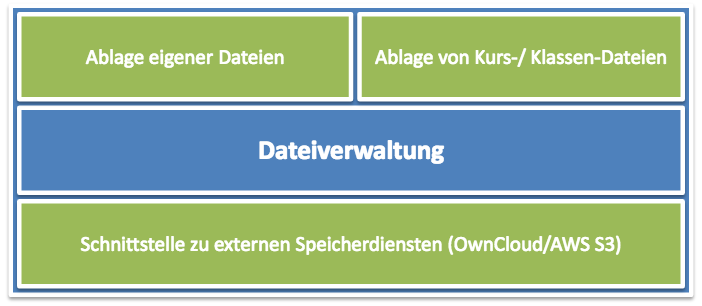
\includegraphics[width=0.8\linewidth]{images/AnforderungenDateiverwaltung}
			\caption[Caption for relatedWork]{Grundanforderungen an die Dateiverwaltung der Schul-Cloud\footnotemark}
			\label{fig:devices}
		\end{center}
	\end{figure}
	\footnotetext{Martin Hense (Mint-EC - \url{https://www.mint-ec.de/})}
\end{center}

\subsection{Grundaufbau Dateiverwaltung}

\subsection{Architektur verteilter Provider}

\subsection{Interaktion verschiedener Schul-Cloud Komponenten}

\subsection{File Sharing}

\clearpage
